\documentclass{beamer}

\usetheme{default}
\setbeamertemplate{navigation symbols}{} % No navigation symbols
\usecolortheme[named=white]{structure} % White titles and such
%\setbeamercolor{normal text}{fg=white} % White text
\setbeamercolor{background canvas}{bg=black} % Black background
% Comment this line for default bullet points (triangles)
\setbeamertemplate{itemize item}{\color{white}$\bullet$} 

\begin{document}

\begin{frame}
\end{frame}

\setbeamercolor{background canvas}{bg=white}

\begin{frame} % Potential pathways from historical states to conflict
	\begin{figure}
		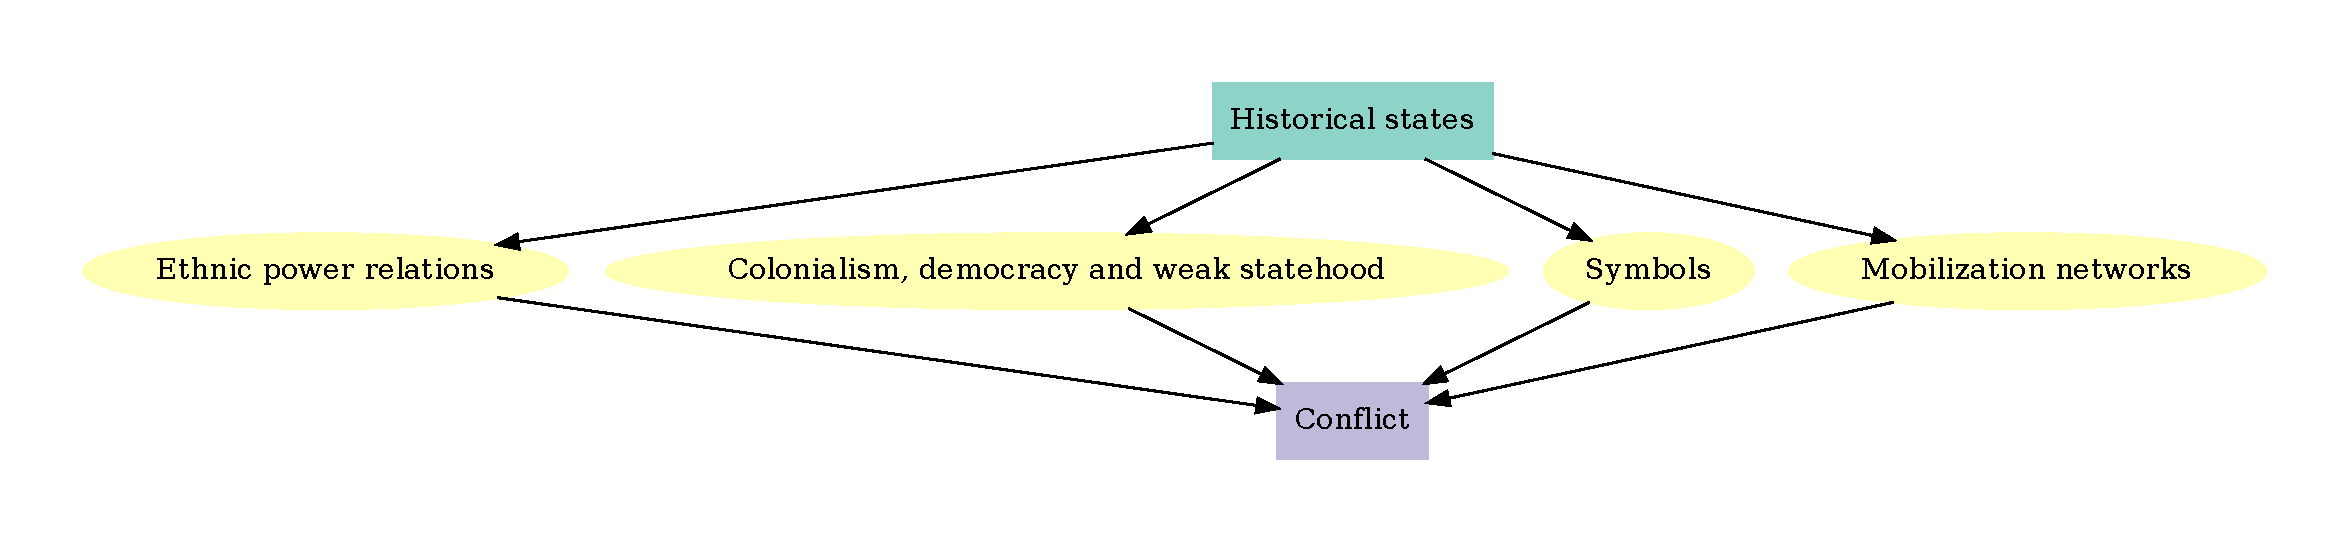
\includegraphics[width=\linewidth]{img/graf.pdf}
	\end{figure}
\end{frame}

\setbeamercolor{background canvas}{bg=black}

\begin{frame}
\end{frame}

\setbeamercolor{background canvas}{bg=white}

\begin{frame} % OMT Causal
	\begin{figure}
		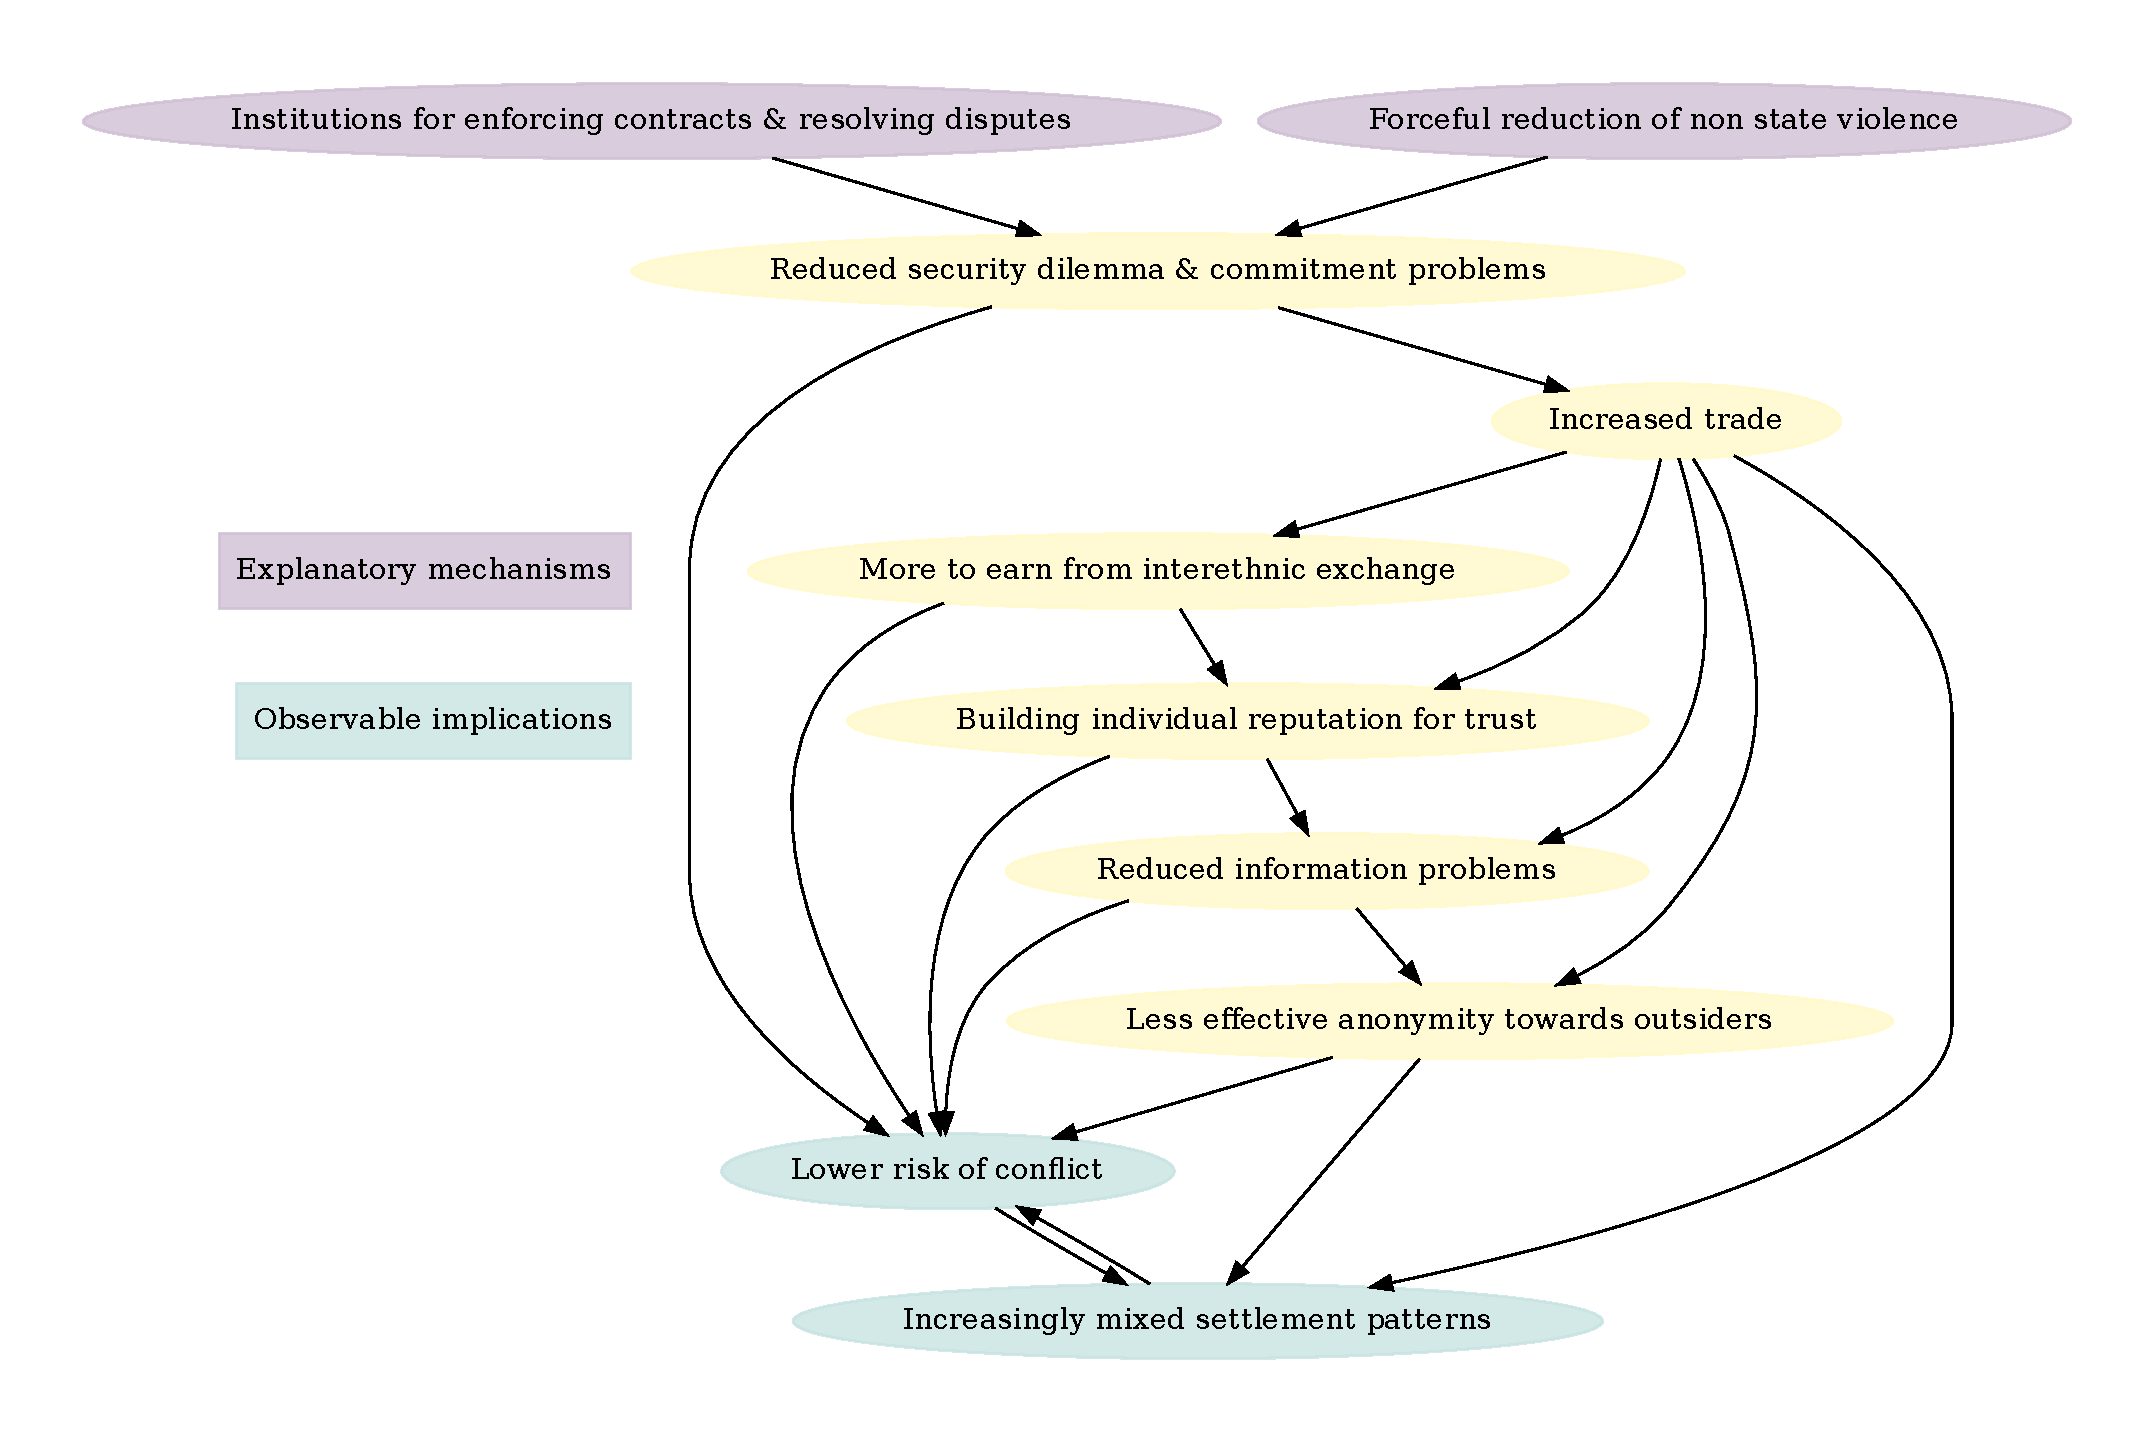
\includegraphics[width=\linewidth]{img/OMTcausal.pdf}
	\end{figure}
\end{frame}

\setbeamercolor{background canvas}{bg=black}

\begin{frame}
\end{frame}

\setbeamercolor{background canvas}{bg=white}

\begin{frame} % ARC
	\begin{figure}
		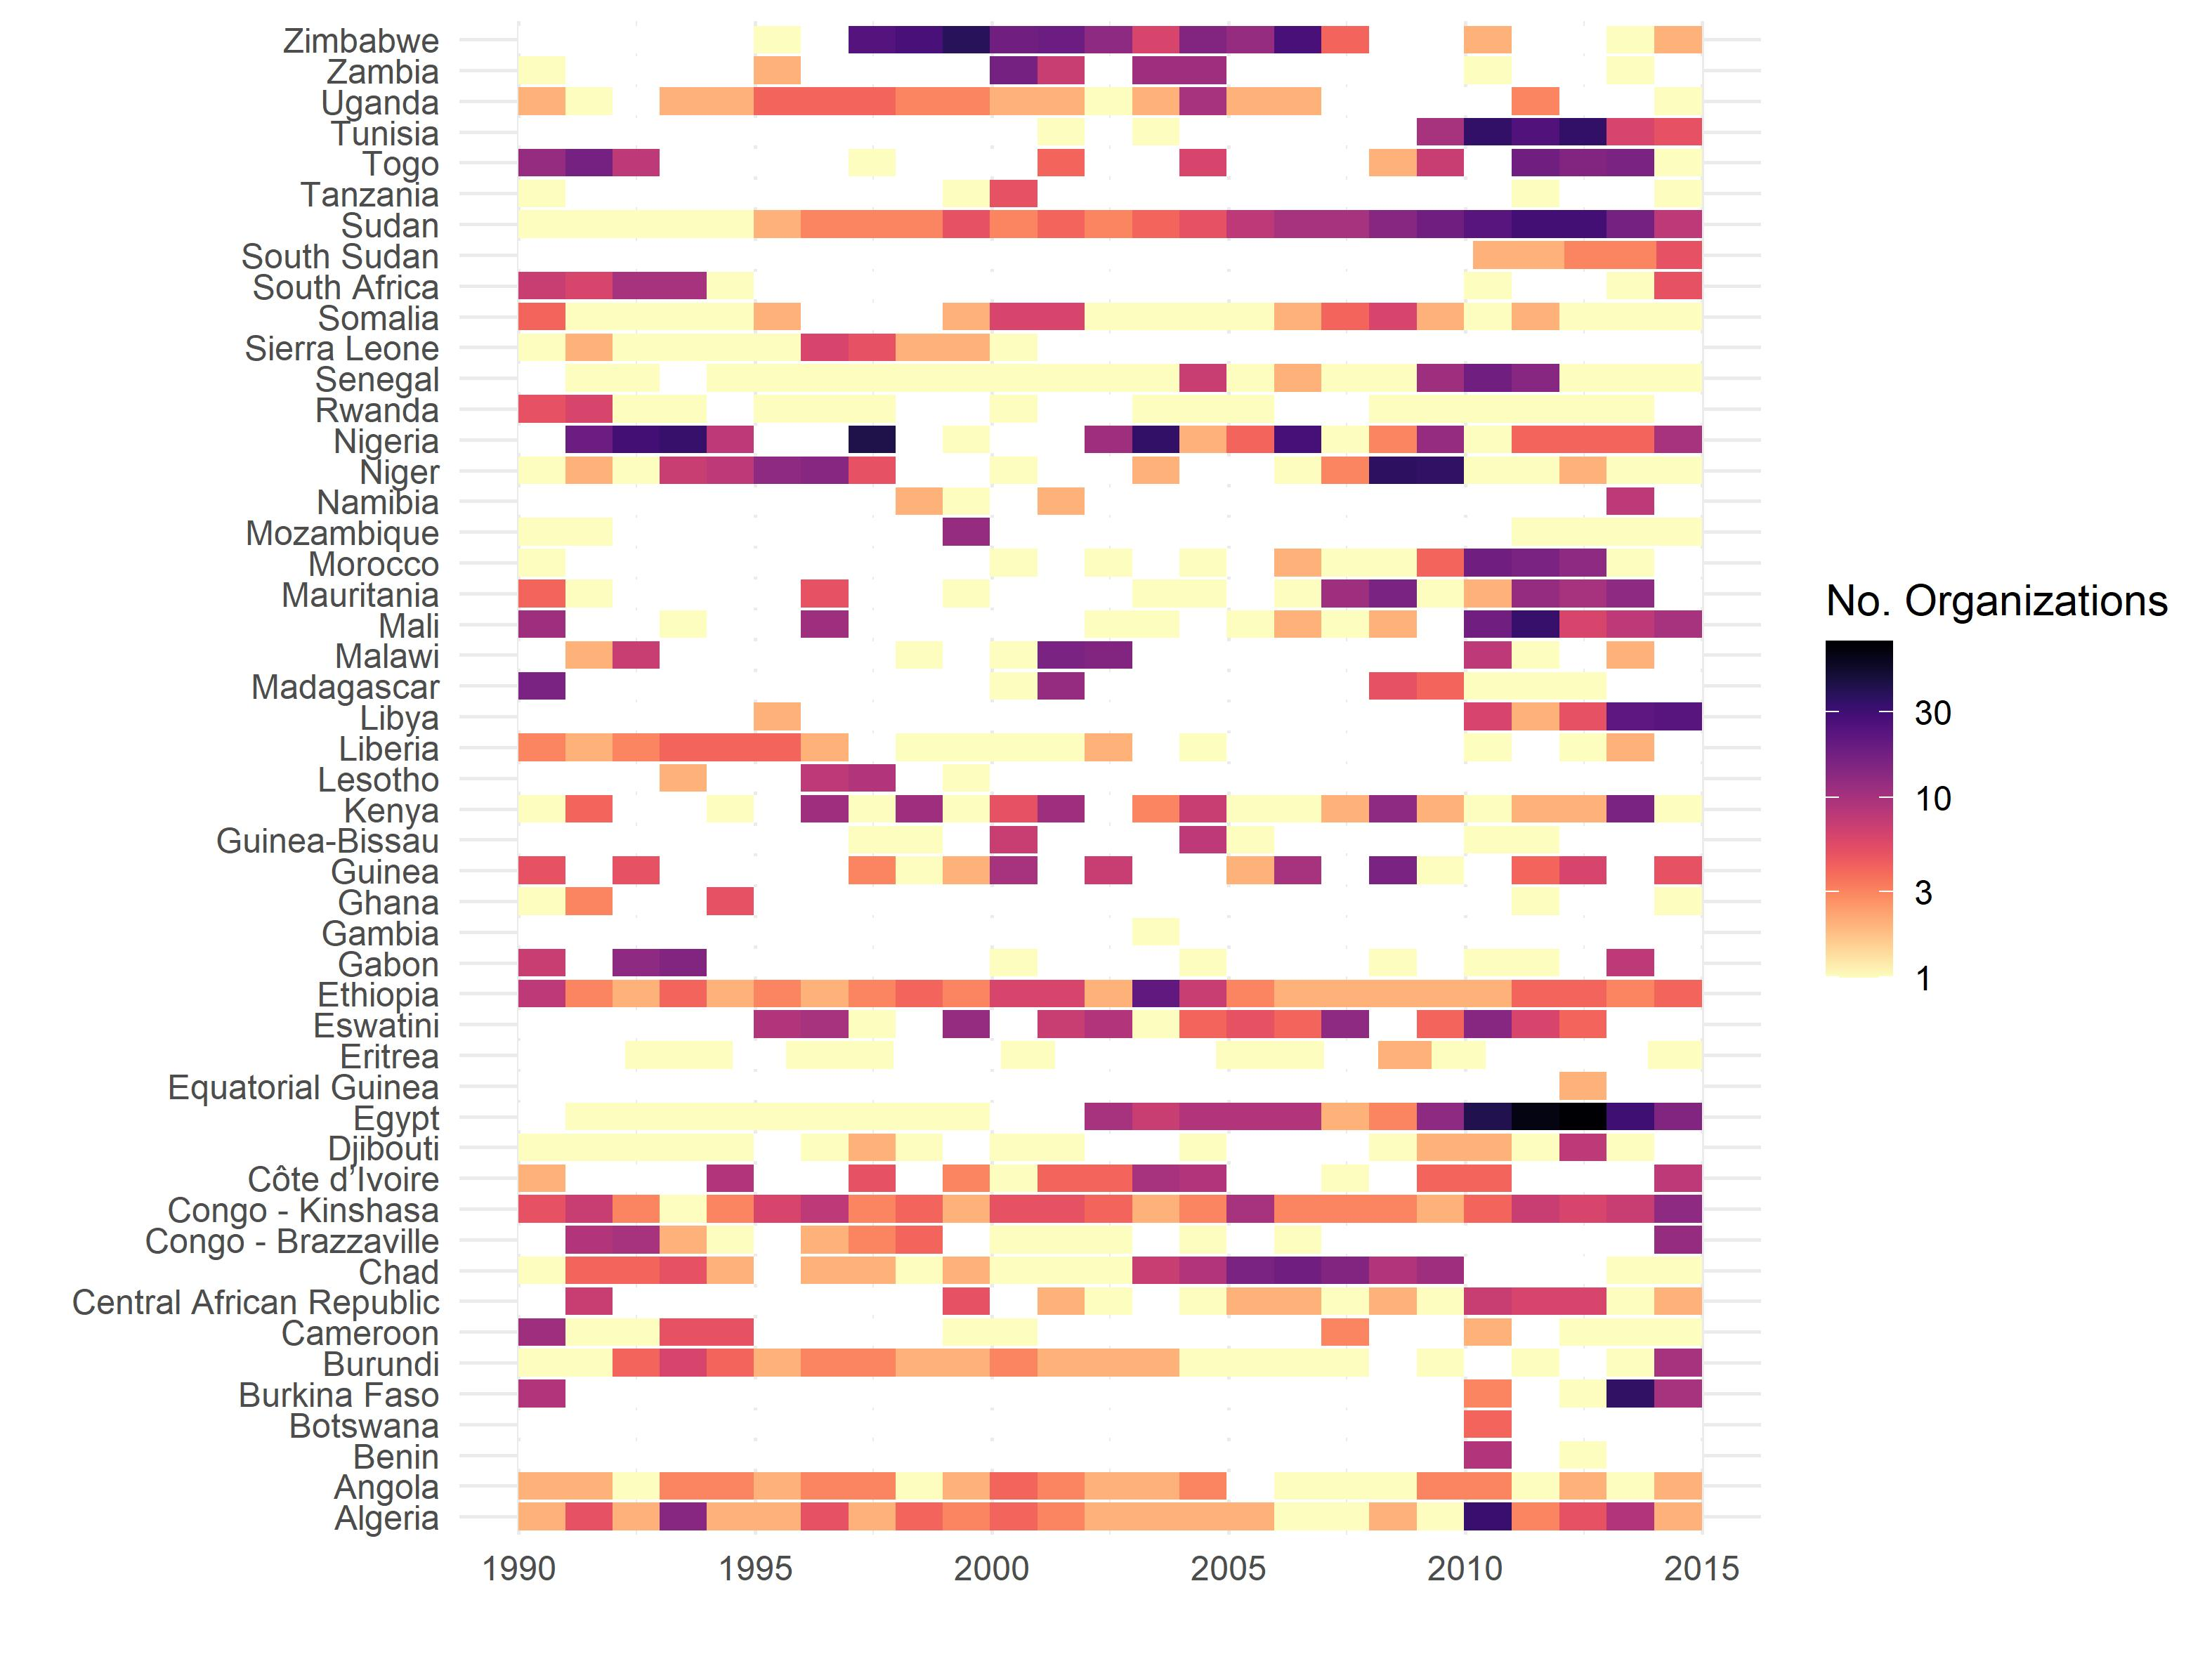
\includegraphics[width=.9\textwidth]{img/figure_2_revised.jpg}
		\caption{ARC organizations over time and space}
	\end{figure}
\end{frame}

\begin{frame} % Geo-ISD
	\begin{figure}
		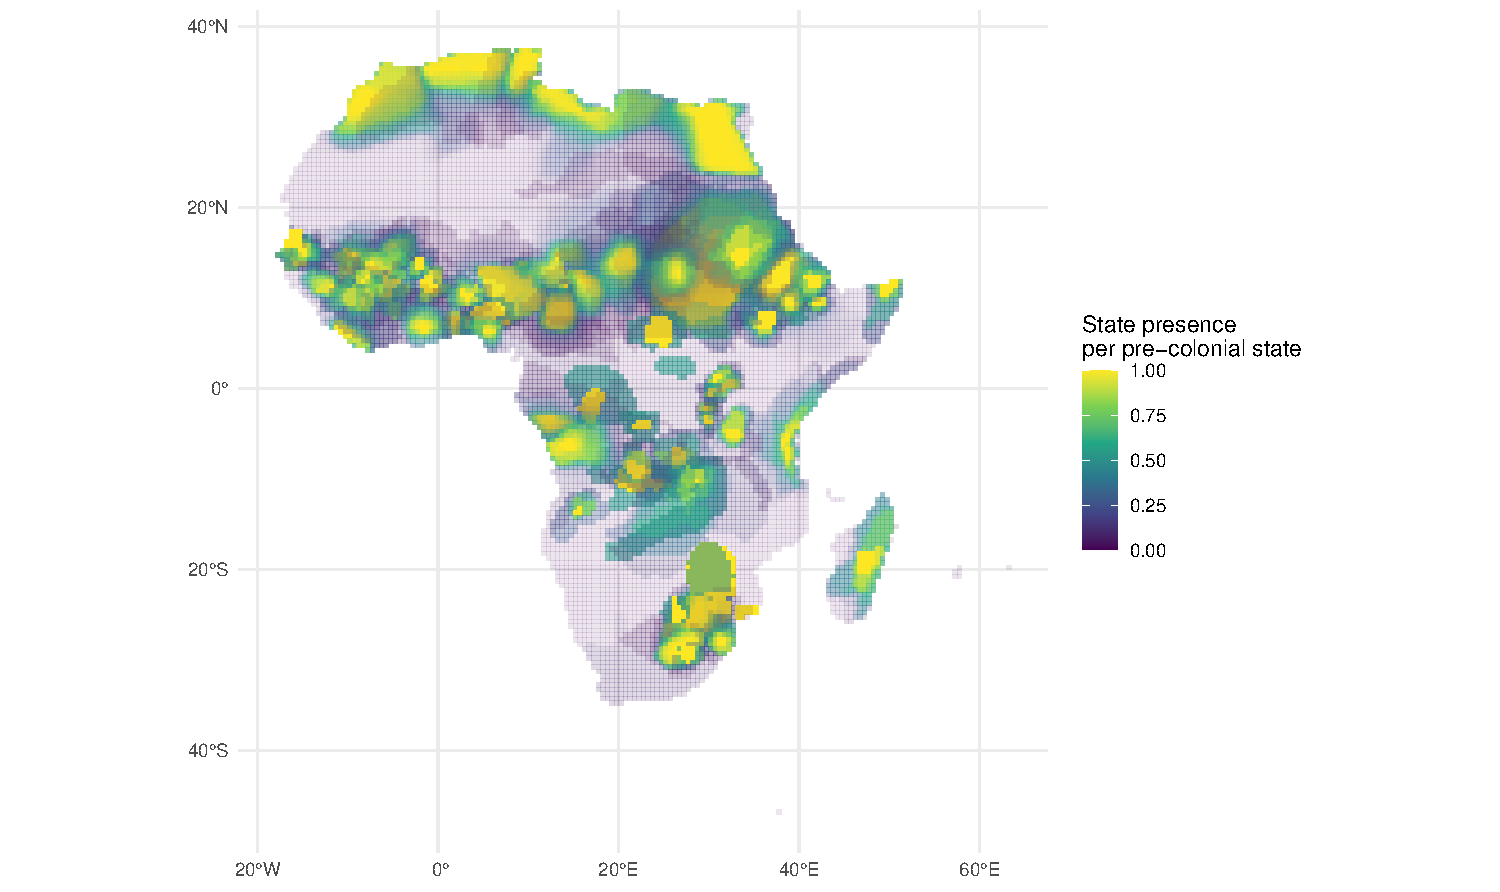
\includegraphics[width=\textwidth]{img/geo_isd_all.pdf}
		\caption{Pre-colonial state presence (normalized per pre-colonial state)}
	\end{figure}
\end{frame}

\begin{frame} % Nigeria
	\begin{figure}
		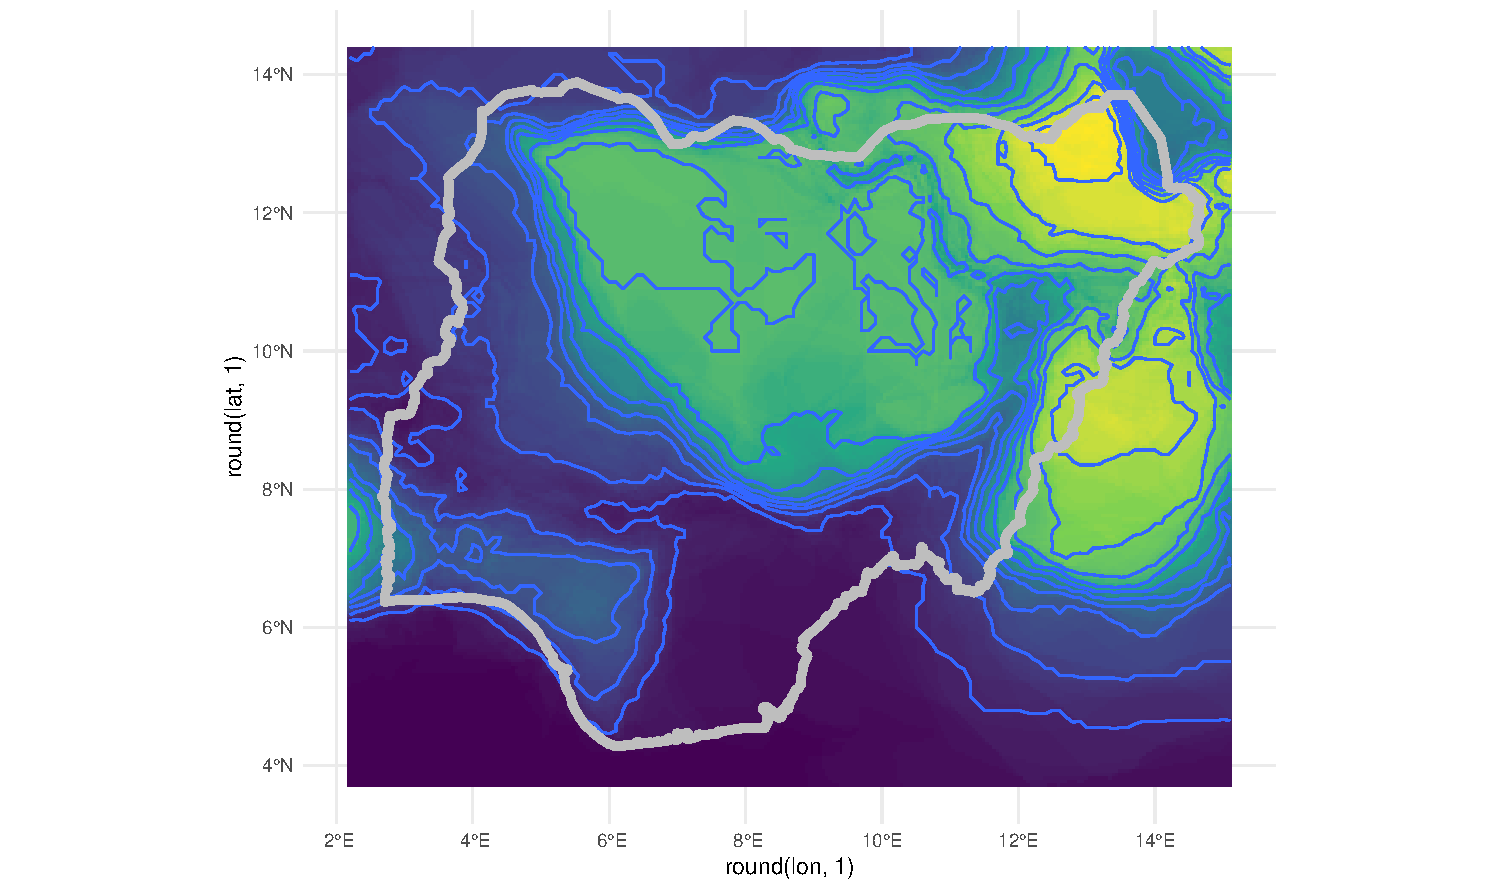
\includegraphics[width=\linewidth]{../R/Output/nigeria.pdf}
	\end{figure}
\end{frame}

\setbeamercolor{background canvas}{bg=black}

\begin{frame}
\end{frame}

\setbeamercolor{background canvas}{bg=white}

\begin{frame} % Beyond Ethnicity
	\begin{figure}
		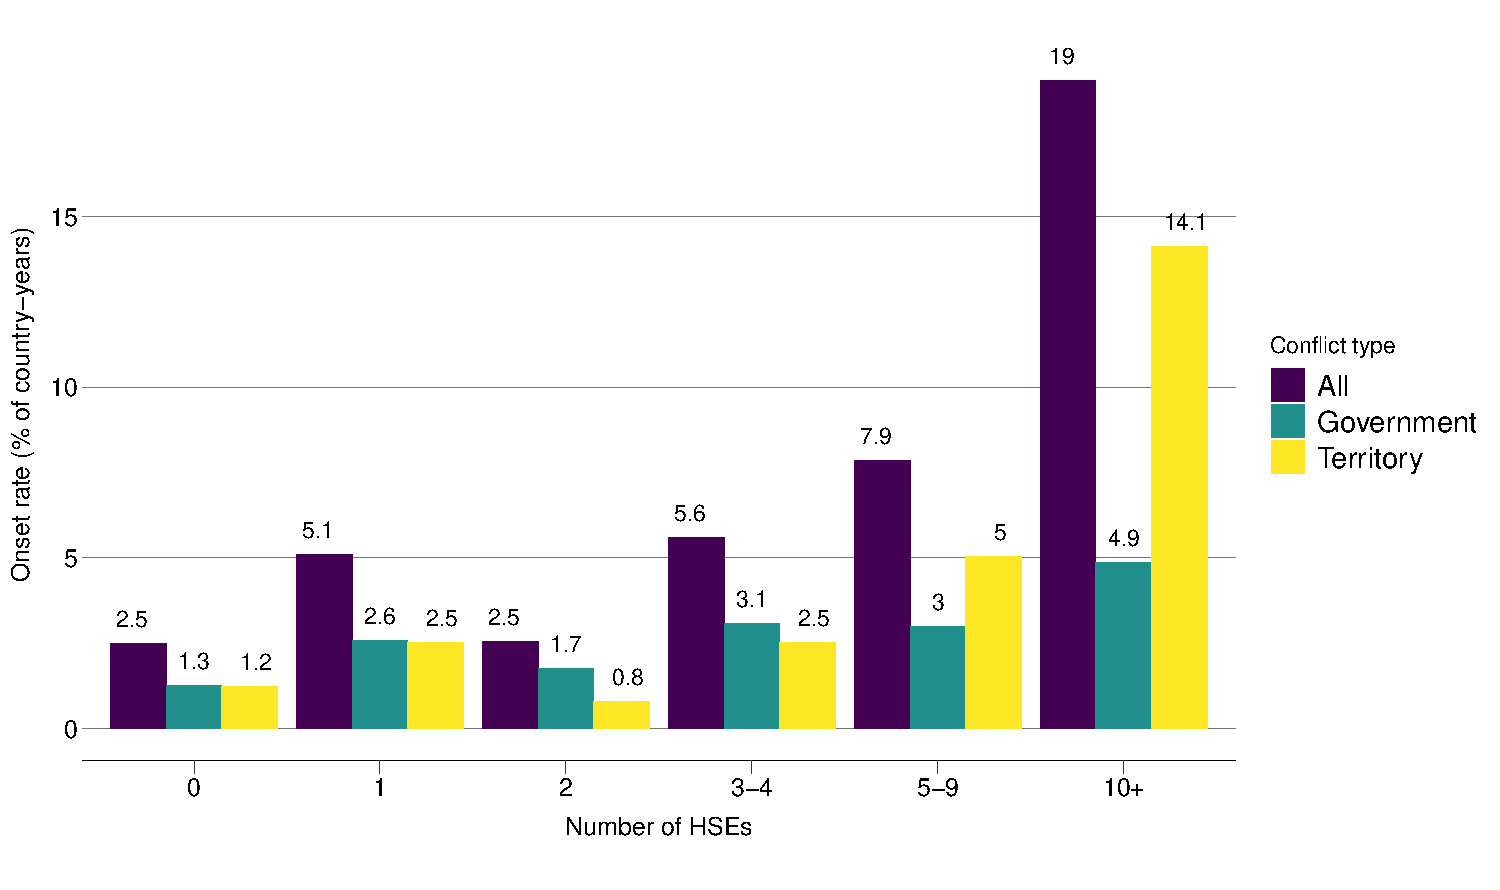
\includegraphics[width=\linewidth]{img/hse_onset_rates.pdf}
	\end{figure}
\end{frame}

\setbeamercolor{background canvas}{bg=black}

\begin{frame}
\end{frame}

\setbeamercolor{background canvas}{bg=white}

\begin{frame} % Uganda
	\begin{figure}
		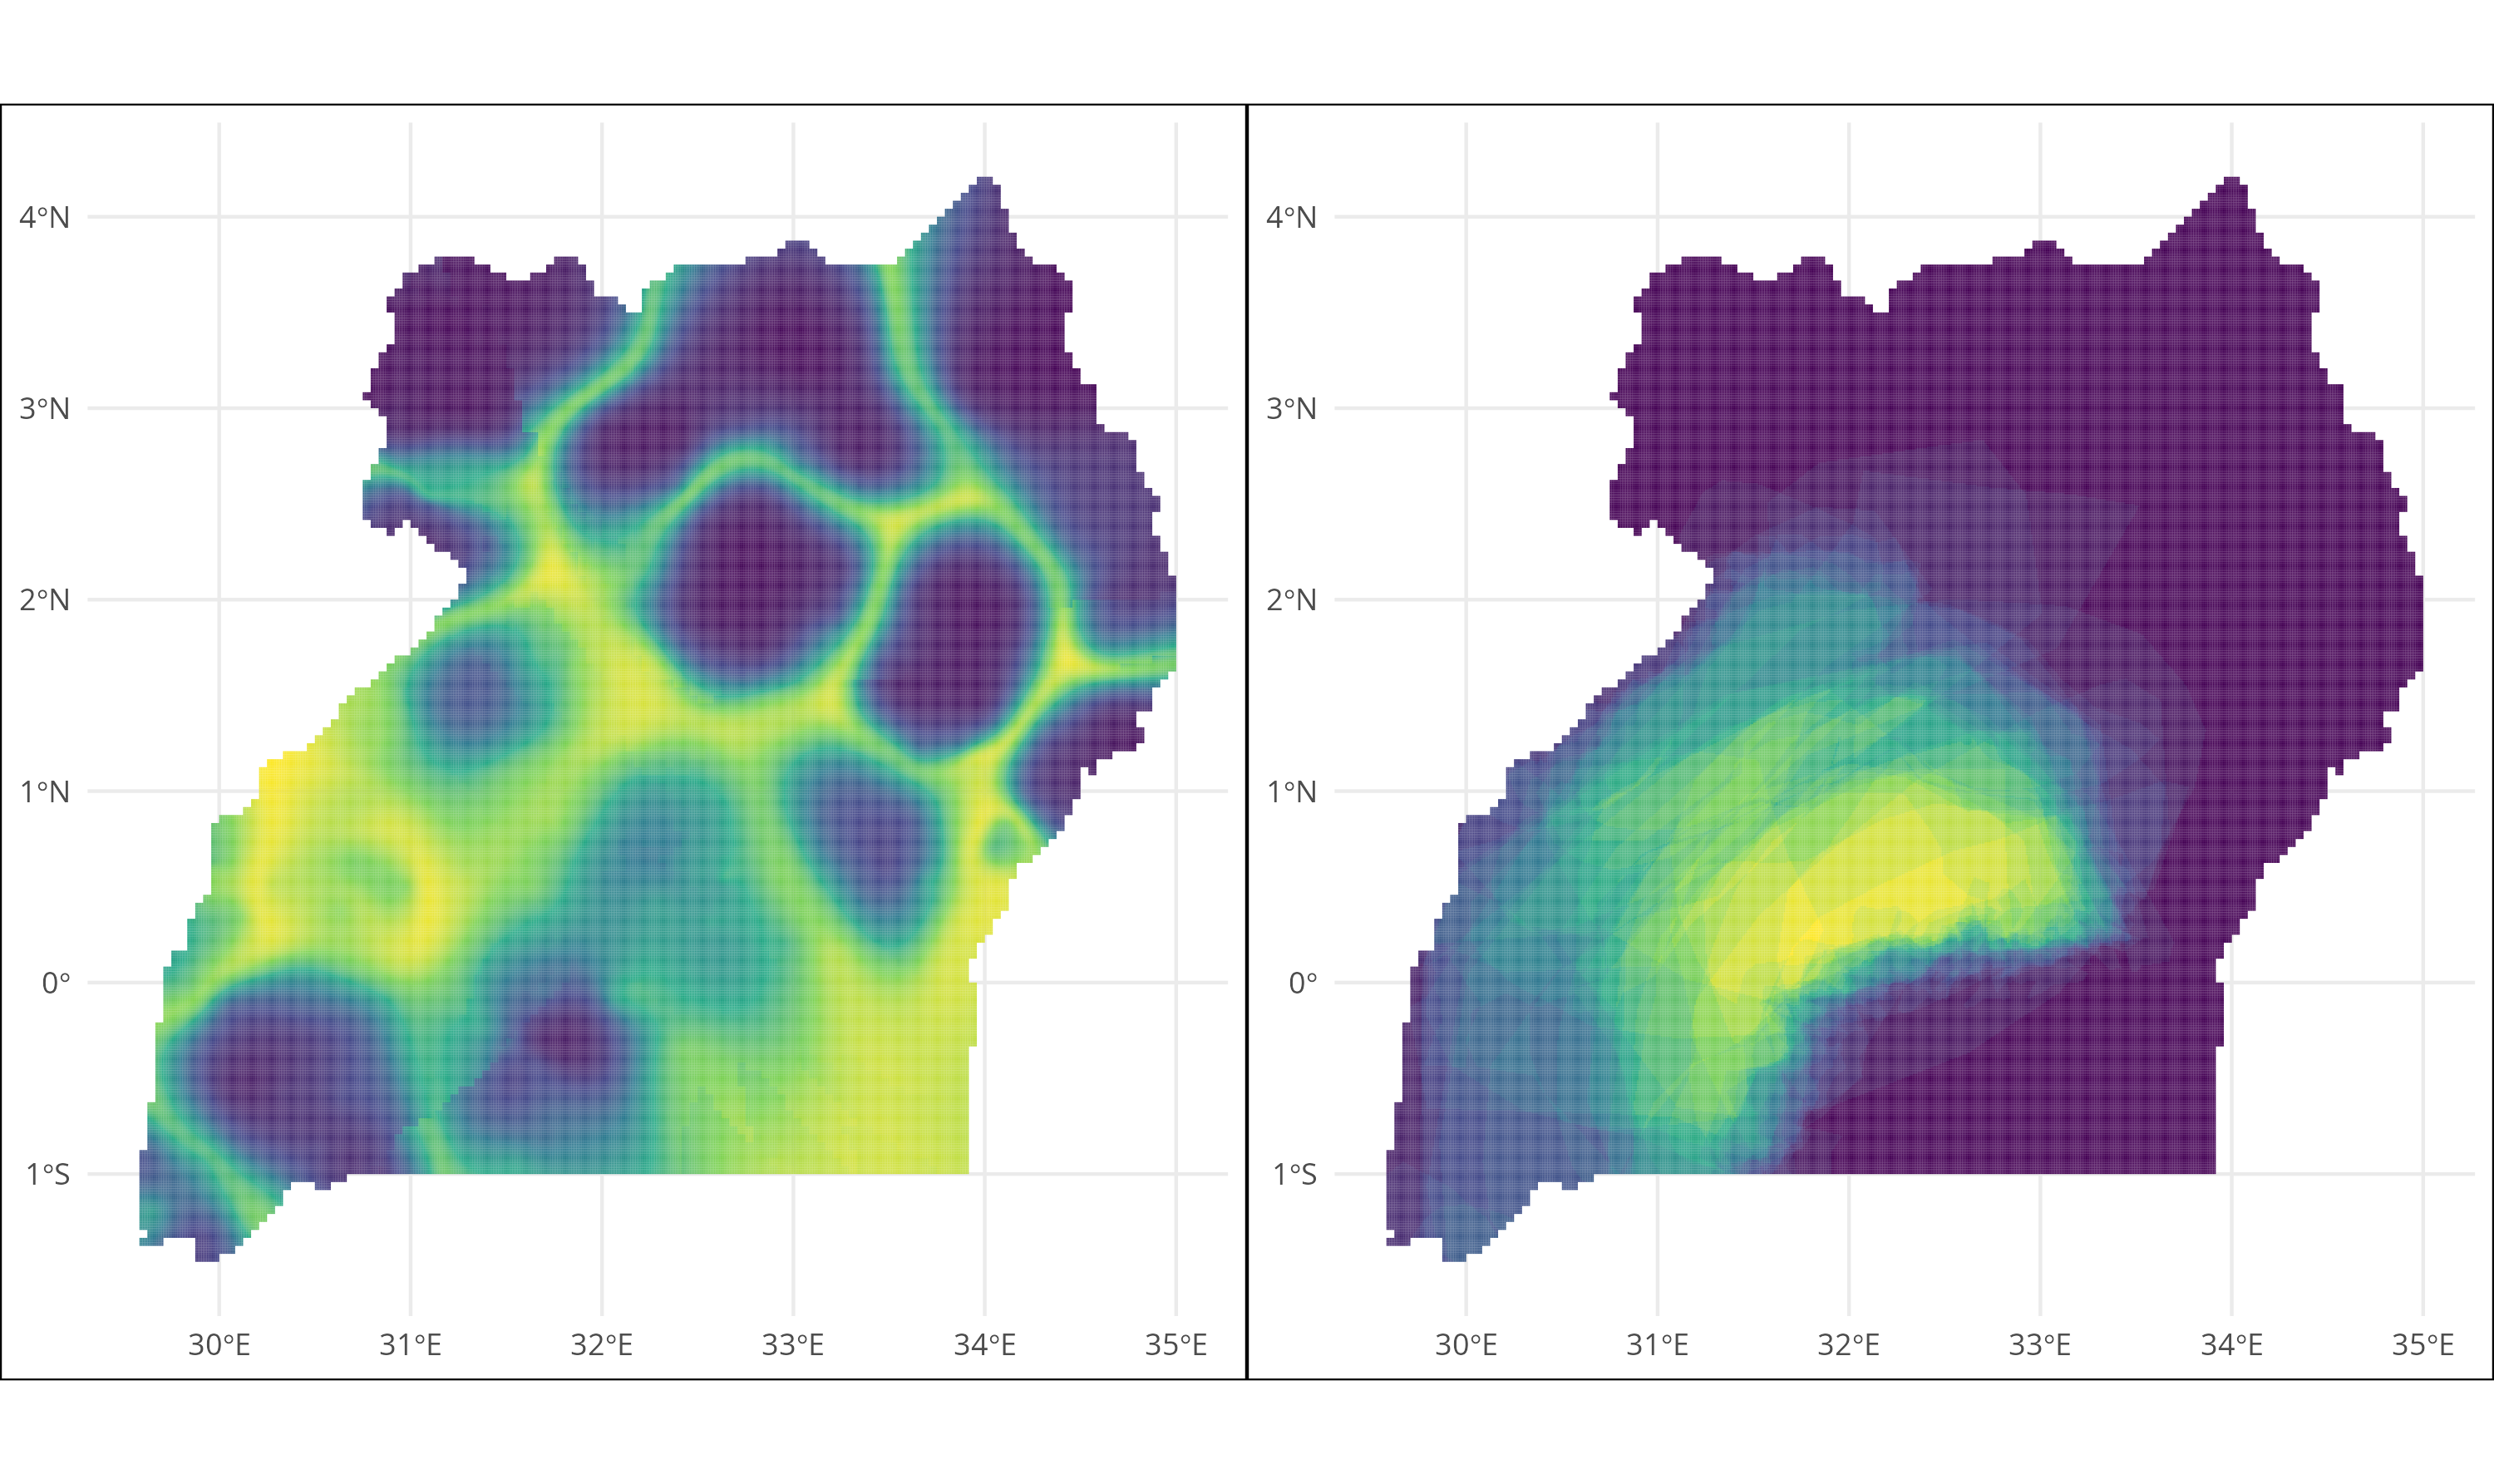
\includegraphics[width=1\linewidth]{img/ugaplots.png}
	\end{figure}
\end{frame}

\setbeamercolor{background canvas}{bg=black}

\begin{frame}
\end{frame}

\setbeamercolor{background canvas}{bg=white}

\begin{frame} % After Forever
	\begin{figure}
		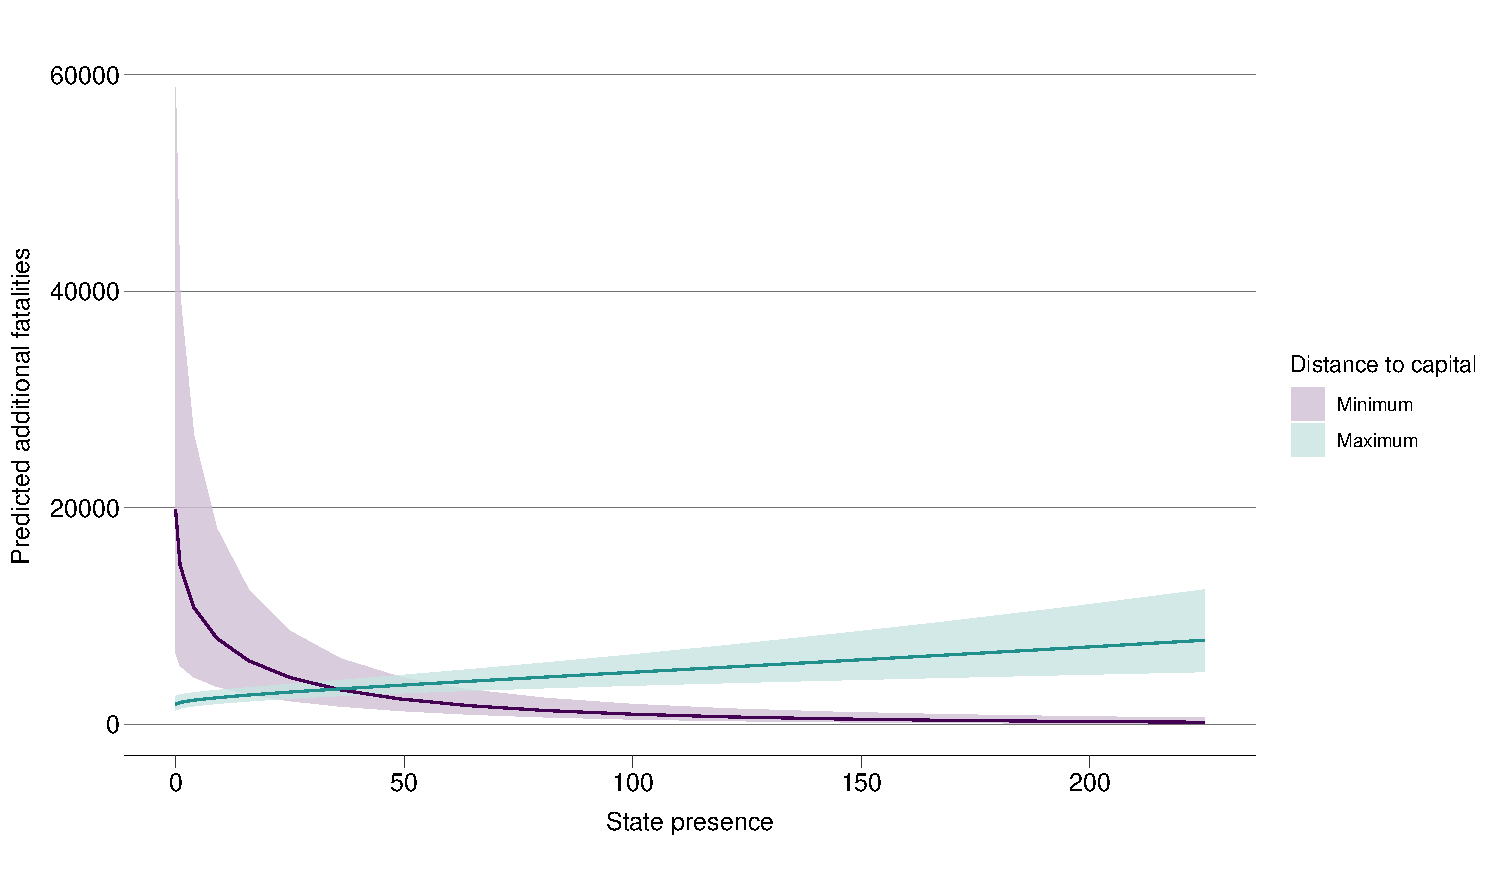
\includegraphics[width=\linewidth]{"../R/Output/interdeathszinbplot.pdf"}
		\caption{Marginal effect of pre-colonial state presence, conditioned on
		distance to capital, in cells with at least one fatality (second stage
		ZINB model).}
	\end{figure}
\end{frame}

\end{document}
